% Yeban User Guide — Chapter 4: The Piano Roll (English)
% T-DOC-001 chapter-by-chapter delivery, written ahead of the CH04 task.
% Sources: app.slint roll properties and menus, help.rs tour, bridge.rs pitch lanes,
% docs/manual/04-piano-roll.md, cli.rs SHORTCUTS.

\chapter{The Piano Roll}
\label{ch:piano-roll}

\begin{quote}
凡音之起，由人心生也。
\end{quote}

Source: Book of Rites, “Record of Music” (《礼记·乐记》). Translation: “All music begins in the human heart.”

Before a note lands on the roll there is an emotion to express; technique and rules serve what is heard.

The piano roll is where MIDI notes are written: time runs horizontally, pitch
vertically. This chapter covers opening it, drawing notes, editing velocity and
quantizing, plus the current limits of note dragging.

\section{Open and Navigate the View}

\subsection{Open the roll}

Press P, or switch to the piano roll — the first bottom-console tab; F7 is the direct
key for that tab. Select a clip on a MIDI synth track and the roll shows the notes in
that clip.

\subsection{Read the two dimensions}

The horizontal axis is time (in ticks, converted to bars/beats from the project's time
signature); the vertical axis is pitch, arranged as pitch lanes from high to low, with
key labels on the left (e.g.\ C4, Eb5) as references. A readout at the top shows the
currently visible pitch range. At the bottom is the velocity lane, where each note's
velocity appears as a vertical bar.

\screenshot{ch04-roll-overview}{The piano roll in full, labelling the time ruler, pitch lanes with key labels and the velocity lane}

\subsection{Zoom and framing}

Cmd/Ctrl+Up/Down zooms tracks vertically; Cmd/Ctrl+=/-- zooms the timeline
horizontally. The roll has a "framing" notion: you can frame the current clip, the
current track or all content. Pitches outside the visible window are not drawn —
change the framing to see them.

\section{Note Entry, Selection and Movement}

\subsection{Draw notes}

The onboarding tour puts it plainly: \textbf{number key 2 is the draw tool}; click on
the roll and a note lands there. The drop position comes from the click: horizontal
for time, vertical resolved from the y coordinate into a pitch lane. Once drawn, drag
the note to change time or pitch, or drag its right edge to change length.

\subsection{Select and drag}

Clicking a note selects it. In the current version pointer dragging acts only on the
note under the pointer — even if several are selected, dragging one leaves the others
where they are. So "group drag" and "group duration change" do not work yet; move
notes one at a time, or wait until the capability officially lands. Yeban does not
disguise an unimplemented operation as a success.

\begin{figure}[htbp]
\centering
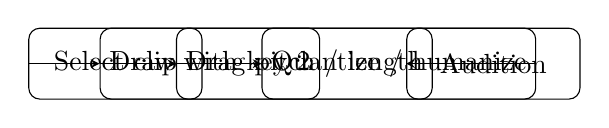
\begin{tikzpicture}[node distance=1.2cm, >=stealth,
    box/.style={draw, rounded corners, align=center, minimum width=2.2cm, minimum height=0.9cm}]
  \node[box] (a) {Select clip};
  \node[box, right of=a] (b) {Draw with key 2};
  \node[box, right of=b] (c) {Drag pitch / length};
  \node[box, right of=c] (d) {Quantize / humanize};
  \node[box, right of=d] (e) {Audition};
  \draw[->] (a)--(b); \draw[->] (b)--(c); \draw[->] (c)--(d); \draw[->] (d)--(e);
\end{tikzpicture}
\caption{Common roll flow: select clip $\to$ draw $\to$ edit pitch/length $\to$ quantize $\to$ audition}
\label{fig:ch04-roll-flow}
\end{figure}

\section{Velocity, Quantize and Scale Tools}

\subsection{Velocity}

In the bottom velocity lane each note has a vertical bar whose height is its velocity.
You can edit a note's velocity directly there; the roll previews the value while
dragging.

\subsection{Quantize and humanize}

Edit $\to$ Note Quantize (Quantize 1/16)... snaps selected notes to a 1/16 grid;
Edit $\to$ Note Humanize... opens a dialog with time jitter, velocity jitter, strength
and seed settings to make mechanical results feel more natural. Both affect only the
current selection.

\screenshot{ch04-humanize-dialog}{The Humanize dialog showing time jitter, velocity jitter and strength inputs}

\subsection{Scale and chord tools}

The current version offers key labels on the pitch lanes as pitch references; whether
standalone scale/chord generation tools exist depends on the build you use — do not
assume an entry that is not present. Edit $\to$ Drum Generation (Drums)... does exist
and can generate a drum clip from style, complexity and seed.

\section{Step Editing and Chord Assistance}

"Step editing" here means writing notes one fixed step at a time: place a note in each
target cell with the draw tool, then use quantize to tidy timing. It is not a
one-click melody generator.

For chords, the available approach is to draw several pitches stacked at the same
moment and verify by ear; automatic chord-progression generation is outside this
chapter's scope and is not described as available.

\section{Help Topic Mapping}

\begin{table}[htbp]
\centering
\caption{Sections of this chapter $\to$ in-app help anchors}
\label{tab:ch04-help}
\begin{tabular}{ll}
\hline
Section & Help topic \\
\hline
Open roll / two dimensions & \texttt{roll-open-view} \\
Zoom and framing & \texttt{roll-zoom-framing} \\
Draw notes and selection & \texttt{roll-note-entry} \\
Select and drag (single-note limit) & \texttt{roll-note-drag} \\
Velocity lane & \texttt{roll-velocity-lane} \\
Quantize and humanize & \texttt{roll-quantize-humanize} \\
Scale tools / step editing & \texttt{roll-scale-step} \\
\hline
\end{tabular}
\end{table}

\paragraph{What you will be able to do} Draw a melody, edit velocity, quantize to 1/16, and explain that dragging currently affects a single note.

\paragraph{Hands-on exercise} Open the roll on a MIDI track clip, draw a one-bar C-major scale with number key 2, make the first note stronger in the velocity lane, quantize with Note Quantize to 1/16, then press Space to audition; finally drag one note and confirm the others stay put.
